\chapter{Estado del arte}\label{cap.estado}

En este capítulo se revisará la bibliografía más relevante relacionada con la monitorización del tráfico obteniendo así información acerca de las diferentes técnicas propuestas. 

Nos centraremos en las técnicas propuestas para la detección, clasificación y seguimiento de vehículos en las cuales se haga uso únicamente de una cámara como sensor. Comentaremos cuales son los métodos empleados, asi como sus ventajas e inconvenientes.

En los últimos años el precio de las cámaras se ha visto reducido y la potencia de cómputo de nuestros dispositivos ha aumentado, favoreciendo al desarrollo de sistemas de análisis de tráfico. Debido a esto, se trata de un área en continuo desarrollo desde los años 90, en el cual se pretende dar una solución en tiempo real. 

En la monitorización del tráfico hay que tener en cuenta tres puntos principales:
\begin{enumerate}
    \item Detección de vehículos
    \item Clasificación de vehículos
    \item Seguimiento de vehículos
\end{enumerate}

La detección consiste en localizar la posición de cada vehículo en la imagen. La clasificación trata de identificar a que clase pertenece cada detección. Y el seguimiento consiste en asociar los vehículos en las sucesivas secuencias de video.

A continuación veremos las soluciones que plantean los diferentes autores para cada punto. Hay que decir que en muchas ocasiones la detección y la clasificación se hacen conjuntamente. No obstante vamos a comentar por separado cada fase.

\section{Detección de vehículos} \label{ap.deteccion_vehiculos}

La detección de vehículos trata de identificar donde se localizan los vehículos en los fotogramas. En la literatura hay numerosas técnicas que han sido planteadas para esta función, las cuales van a ser comentadas a continuación. 

Una técnica muy empleada en este problema es la sustracción del fondo. Se trata de restar la imagen del fondo de las sucesivas imágenes, con el fin de quedarnos con los objetos que se encuentran en movimiento, que en este caso en concreto serán los vehículos. S.I. Arroyo, F. Safar y D. Oliva ~\cite{probabilidad_infraccion}
 se basan en la diferencia entre el fotograma actual y la imagen referencia (imagen de fondo). Esta imagen referencia debe ajustarse a las condiciones de luminosidad en el tiempo.
 
 Otra técnica muy parecida a la sustracción de fondo es la diferencia absoluta (SAD) entre dos secuencias. A.F. Granados y J.I. Marin .H~\cite{deteccion_flujo_vehicular} presentan una técnica basada  en la diferencia absoluta (\acrfull{sad}) entre dos secuencias. Para ello aplican filtrado homomórfico con el fin de reducir el efecto de los cambios de iluminación. Tras esto realizan la diferencia absoluta (\acrshort{sad}), umbralizan y segmentan los objetos en movimiento. J. Portillo, G. Sánchez, J. Olivares y H. Pérez~\cite{deteccion_movimiento} también propusieron un método en el que se hacía uso de la \acrshort{sad} y complementariamente se realizaba un análisis de bordes en la región considerada en movimiento.

En la vida real tenemos situaciones más complejas, pues los cambios de iluminación y la aparición de objetos en la escena (por ejemplo ramas de los árboles, personas, etc) es muy probable. Por tanto, necesitamos un método que sea capaz de funcionar correctamente a pesar de estos problemas.

\acrfull{mog} es una técnica que aplicaron C.Stauffer and  W.E.  Grimson~\cite{adaptative_background} por primera vez al problema de la sustracción de fondo. Esta técnica se basa en el empleo de varias gaussianas para modelar cada píxel, permitiendo modelar varios estados del fondo a un mismo píxel. Es decir, esta técnica permite modelar un píxel cuyo valor cambia constantemente debido a movimientos periódicos.  La probabilidad actual de un píxel se calcula en función de los valores que ha tomado a lo largo de un tiempo X\textsubscript{1},...,X\textsubscript{t} mediante la fórmula:

\begin{equation}\label{gmm_formula}
P(X_{x}) = \sum_{i=1}^{k}\omega_{i,t}*\eta(X_{t},\mu_{i,t},\Sigma_{i,t}) 
\end{equation}

Donde \textit{k} es el número de gaussianas, $\eta$ es  una  gaussiana  de  media $\mu$\textsubscript{i,t} y cuya matriz de covarianza es $\Sigma$\textsubscript{i,t}. El valor $\omega$\textsubscript{i,t}, es una estimación de su peso y puede variar con el tiempo (hace referencia a la proporción que supone esta gaussiana en la decisión final). La función de densidad de probabilidad $\eta$ tiene la siguiente forma:

\begin{equation}\label{eta_formula}
\eta(X_{t},\mu,\Sigma) = \frac{1}{(2\pi)^{\frac{n}{2}}|\Sigma|^{\frac{1}{2}}}e^{-\frac{1}{2}(X_{t}-\mu_{t})^{T}\Sigma^{-1}(X_{t}-\mu_{t})}
\end{equation}

El número de gaussianas \textit{k} viene determinado por el número de \textit{modos} posibles para el fondo, los cuales dependen del escenario. Este número afecta de forma directa  al  tiempo  de  procesamiento. En una implementación básica de \acrshort{mog} se  asume que los canales (R,G,B) son independientes, obteniendo de esta forma una matriz de covarianza reducida:

\begin{equation}\label{covarianza_formula}
\Sigma_{k,t}=\sigma_{k}^2I
\end{equation}

En esta versión de \acrshort{mog} la pertenencia de cada nuevo píxel al fondo es evaluada contra las distintas gaussianas que lo forman. Si el valor de un píxel está en un rango de 2.5 la desviación estándar de la gaussiana se considera que pertenece a dicha gaussiana. El nuevo píxel será clasificado como fondo si pertenece a alguna de estas gaussianas y los parámetros $\mu$\textsubscript{k,t},$\Sigma$\textsubscript{k,t}\textsuperscript{2} y $\omega$\textsubscript{k,t} serán actualizados con el nuevo valor mediante las siguientes fórmulas:

\begin{equation}\label{gaussiana_formula1}
\omega_{k,t}=(1-\alpha)\omega_{k,t-1}+\alpha(M_{k,t})
\end{equation}
\begin{equation}\label{gaussiana_formula2}
\mu_{t}=(1-\rho)\mu_{t-1}+\rho(X_{t})
\end{equation}
\begin{equation}\label{gaussiana_formula3}
\sigma^2=(1-\rho)\sigma_{t-1}^2+\rho(X_{t}-\mu_{t})^T(X_{t}-\mu_{t})
\end{equation}

Donde $\rho$ se corresponde con:

\begin{equation}\label{ro_formula}
\rho=\alpha\eta(X_{t}|\mu_{k},\sigma_{k})
\end{equation}

M\textsubscript{k,t} vale 1 para la gaussiana que describe el píxel y 0 para el resto. El valor de $\mu$ y $\sigma$ no cambia para el resto de distribuciones. $\alpha$ es el factor de aprendizaje.

Tras esto, los valores de $\omega_{k,t}$ se normalizan entre las \textit{k} distribuciones que modelan al píxel. Si  el píxel  no  pertenece  a  ninguna  de  las  distribuciones,  la  distribución  de menor peso será remplazada por otra con una varianza inicial grande, una media igual al valor del nuevo píxel y un peso inicial bajo.

Lo normal es que no todas las gaussianas sean empleadas para formar parte del modelo de un píxel, sino que se escoge un número \textit{T} de gaussianas para formarlo. Debido a los grandes cambios que puede sufrir el fondo no todas las gaussianas que formen parte del modelo representarán algún modo del fondo.

Para realizar todo este proceso se ordenarán las distribuciones en función del valor de $\omega$/$\sigma$. Los componentes con un alto peso en la mezcla de gaussianas y poca desviación serán los primeros en ser utilizados a la hora de evaluar la pertenencia de un píxel al fondo.

La mezcla de gaussianas es muy utilizada en detecciones de fondo, esto se puede ver reflejado en la cantidad de trabajos que hacen uso de esta técnica. De hecho el trabajo del que se ha partido en este caso~\cite{redo_tesis} hace uso de una versión mejorada de \acrshort{mog} propuesta por Zoran Zivkovic~\cite{zoran_zivkovic}. El avance de este método es que para cada píxel se puede adaptar el número de gaussianas que se van a emplear.


P. Barcellos, C. Bouvié, F.L. Escouto and  J. Scharcanski~\cite{gmm_mei_article} propusieron un método para la detección de vehículos que se basaba en una combinación de \acrfull{gmm} y \acrfull{mei}~\cite{mei_article}. \acrshort{mei} es la imagen de energía de movimiento e indica en cuales píxeles se detecto movimiento a lo largo de una secuencia de fotogramas. Esta técnica se incluye para introducir información temporal del primer plano, ya que gracias a ello tendremos una máscara binaria con los píxeles del primer plano que han sufrido movimiento.

Xia et al.~\cite{gmm_em_article} combinaron \acrshort{gmm} y \acrfull{em}. \acrshort{em} comienza prediciendo los parámetros de las distribuciones y los usa para calcular las probabilidades de que cada objeto pertenezca a una clase. Esas probabilidades se usan para re-estimar los parámetros de las probabilidades hasta que consigamos que converjan. 

Buch et al.~\cite{3dhog_article}  presentaron un sistema que combina  puntos de interés 3D y HOG para detectar el fondo presentando así 3DHOG.


Bjorn Johansson, Johan Wiklund, Per-Erik Forssén and Gösta  Granlund~\cite{combining_shadow} emplean el método estadístico de J.Wood~\cite{wood} para identificar si un píxel pertenece al fondo o al primer plano. El método es una modificación del conocido método de sustracción de fondo de  C.Stauffer and  W.E.  Grimson~\cite{adaptative_background}, con una regla de actualización algo diferente y un límite de regularización más bajo para las desviaciones estándar de Gauss. Principalmente lo que se hace es usar un modelo de mezcla de gaussianas en cada píxel para estimar la distribución de color a lo largo del tiempo, detectándose como píxeles de primer plano aquellos cuyo color sea improbable que pertenezca a la distribución. Además los píxeles de primer plano pueden ser clasificados como sombras. Si el color de un píxel se encuentra en una región cilíndrica entre el negro (el origen) y cualquiera de los colores centrales de los gaussianos de fondo se considerará sombra.


Otra técnica empleada a la hora de detectar el fondo es hacer uso de los denominados \textit{codebooks}. Originalmente esta clase de técnicas fueron empleadas en la clasificación de texto. A la hora de clasificar texto es muy importante disponer de un diccionario de palabras que se ajuste al contenido que tendrá dicho texto. Estas palabras forman lo que se llama  \textit{codebooks} o vocabulario. Este mismo planteamiento se puede emplear a la hora de clasificar imágenes, pero en lugar de palabras tendremos vectores de elementos que describen las características de dichas imágenes.
En este caso se está planteando esta técnica para la detección del fondo pero por supuesto se puede usar a la hora de clasificar los propios vehículos. Al ser una técnica no paramétrica estas palabras no pueden asociarse con distribuciones gaussianas. Hay que decir que este planteamiento no es muy usado en la detección de fondo.

K. Kim, T.H. Chalidabhongse, D. Harwood and L. Davis~\cite{real_time_foreground_background} dicen que 6 palabras son suficientes para clasificar un píxel. Como palabra los autores han empleado un vector RGB $\upsilon i$ = (R\textsubscript{i}, G\textsubscript{i}, B\textsubscript{i}) y una tupla $aux$\textsubscript{i} = [$I$\textsubscript{min}, $I$\textsubscript{max}, $f$\textsubscript{i}, $\lambda$\textsubscript{i}, $p$\textsubscript{i}, $q$\textsubscript{i}] donde:

\begin{itemize}
    \item $I$\textsubscript{min}, $I$\textsubscript{max}: es el mínimo y máximo valor del brillo, para cada píxel asignado a una palabra.
    \item $f$\textsubscript{i}: es la frecuencia con la cual aparece una palabra.
    \item $\lambda$\textsubscript{i}: se trata del máximo intervalo en el cual no ha aparecido la palabra.
    \item $p$\textsubscript{i}, $q$\textsubscript{i}: es la primera y la última vez respectivamente que ha aparecido la palabra.
\end{itemize}

Gracias a $\lambda$\textsubscript{i} podemos saber que valores pertenecen o no al fondo. Si se tiene un valor grande de $\lambda$\textsubscript{i} quiere decir que el objeto en cuestión aparece cada mucho tiempo. Esto puede indicar que se trate de un objeto que ha aparecido de forma temporal y por tanto no pertenece al fondo. Para estimar el fondo se comparará cada píxel de la nueva imagen con la palabra cuya media es más cercana. Si el píxel pertenece a la palabra, querrá decir que pertenece al fondo y por tanto se actualizará la palabra en cuestión con esta nueva información. Si por el contrario, no perteneciera a la palabra se trataría de un objeto en movimiento.

En el planteamiento de M. Mazaheri and S. Mozaffari~\cite{real_time_adaptative_background} la detección esta basada en \textit{codebooks}.

Otro de los métodos empleados en la detección de fondo son los basados en la estimación no paramétrica de la función de densidad a partir de un número de muestras determinadas. Un caso muy popular de este método son los histogramas, los cuales representan la frecuencia de cada valor de forma gráfica a través de barras. Con ello se puede ver la distribución de los datos. Esto tiene un problema y es que en función del rango de la cuantización el resultado puede variar. Para evitarlo, se hace uso de una función matemática llamada \textit{núcleo}, que obtiene una representación más suave de los datos. Dado un conjunto de valores de entrada (X\textsubscript{1},X\textsubscript{2},...,X\textsubscript{n}), los cuales vienen de una distribución desconocida \textsubscript{f}, su \textit{núcleo} se calcula de la siguiente forma:

\begin{equation}\label{nucleo_formula}
\widehat{f}_{h}(x) = \frac{1}{n}\sum_{i=1}^{n}K_{h}(x - x_{i}) = \frac{1}{nh}\sum_{i=1}^{n}K(\frac{x - x_{i}}{h})
\end{equation}

\textit{K} es una función no negativa que integra a uno. La \textit{h} es el \textit{ancho de ventana} y siempre toma valores positivos. 
A. Elgammal, D. Harwood and L. Davis~\cite{non_parametric_model} han aplicado este método para la estimación del fondo. En concreto plantean como \textit{núcleo} una gaussiana N(0,$\Sigma$), donde $\Sigma$ hace referencia al \textit{ancho de ventana}. Por tanto la ecuación \ref{nucleo_formula} quedará de la siguiente manera:

\begin{equation}\label{nucleo_formula_new}
{P}_{r}(x_{t}) = \frac{1}{N}\sum_{i=1}^{N}\frac{1}{(2\pi)^\frac{d}{2}|\Sigma|^\frac{1}{2}} e^{-\frac{1}{2}(x_{t}-x_{i})^{T}\Sigma^{-1}(x_{t}-x_{i})}
\end{equation}

Si asumimos que el ancho de ventana $\sigma$\textsubscript{j} es distinto para cada canal porque los canales de color son independientes tenemos que $\Sigma$ es:

\begin{equation}\label{matriz_sigma}
   \Sigma = \begin{bmatrix}
            \sigma_{1}^2 & 0 & 0 \\
            0 & \sigma_{2}^2 & 0 \\
            0 & 0 & \sigma_{3}^2 \\
\end{bmatrix}
\end{equation}

Quedando la función de densidad como:

\begin{equation}\label{funcion_densidad}
{P}_{r}(x_{t}) = \frac{1}{N}\sum_{i=1}^{N}\prod_{j=1}^{d}\frac{1}{\sqrt{2\pi\sigma_{j}^2}} e^{-\frac{(x_{tj}-x_{ij})^2}{2\sigma_{j}^2}}
\end{equation}

En función del valor de $P_{
r}(x_{t})$ podemos saber si el píxel pertenece a un objeto en movimiento o no. Si  $P_{
r}(x_{t})$ se encuentra por debajo de un umbral fijado consideraremos que se trata de un píxel perteneciente a un objeto en movimiento.
\\

Todas las técnicas que se han ido comentando a lo largo de esta sección basan la detección de vehículos en la detección del fondo. En función de este fondo pueden saber cuales son los objetos que se encuentran en movimiento. Actualmente ha tomado mucha popularidad el deep learning, gracias a lo cual podemos ser capacez de detectar objetos con grandes resultados, sin necesidad de tener que detectar el fondo. 

Rigoberto Vizcay~\cite{tesis_rigoberto} se basa en redes \acrshort{cnn} para la detección de vehículos y peatones. Una red neuronal convolucional es una red que presenta una o varias capas convolucionales.

Y. Abdullah, G. Mehmet, A. Iman and B. Erkan~\cite{rcnn_detection}  plantean el uso de fast \acrfull{rcnn}r y \acrfull{rcnn} para la detección de vehículos. 
\\

\acrshort{rcnn} para realizar las detecciones realiza tres fases:
\begin{enumerate}
    \item Se emplear el algoritmo Selective Search, el cual solo realiza las pruebas de detección a las regiones candidatas a tener una posible detección. Con ello se extraen aproximadamente 2000 regiones de la imagen (Region Proposal).
    \item Se implementa una red neuronal \acrfull{cnn} en la parte superior de cada región.
    \item Se extrapola la salida de cada \acrshort{cnn} y se ingresa en una \acrfull{svm} para clasificar la región. Además se realiza una regresión lineal para restringir el cuadro de la detección.
\end{enumerate}

Estas fases pueden verse en la Figura ~\ref{fig.rcnn}.

\begin{figure}[H]
  \begin{center}
    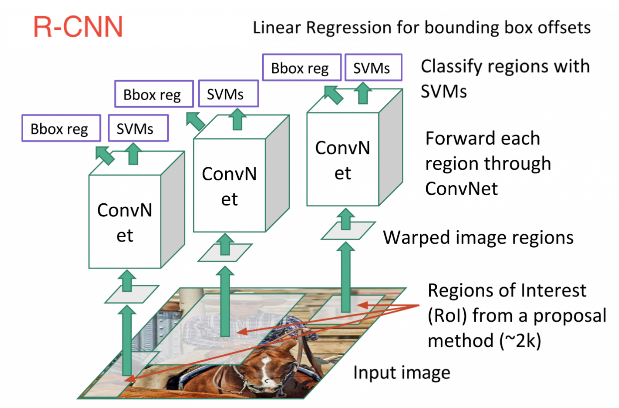
\includegraphics[width=0.7\textwidth]{figures/Estado_arte/rcnn.png}
		\caption{Fases de \acrshort{rcnn}}
		\label{fig.rcnn}
		\end{center}
\end{figure}

Fast \acrshort{rcnn} es una versión más rápida que \acrshort{rcnn}, en la que se modifican algunos aspectos para conseguirlo:
\begin{enumerate}
    \item Antes de extraer las regiones de interés se extraen las características. Para ello se emplea una única \acrshort{cnn} para toda la imagen en vez de 2000.
    \item \acrshort{svm} se remplaza por la función de softmax.
\end{enumerate}

\begin{figure}[H]
  \begin{center}
    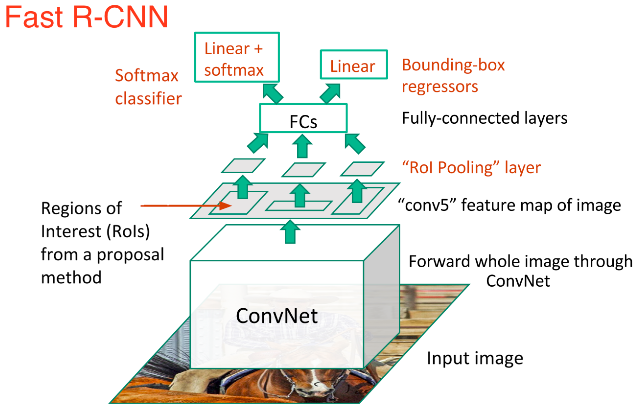
\includegraphics[width=0.7\textwidth]{figures/Estado_arte/fast_rcnn.png}
		\caption{Fases de Fast \acrshort{rcnn}}
		\label{fig.fast_rcnn}
		\end{center}
\end{figure}

Ignacio Arriola~\cite{tesis_ignacio_arriola} hace uso de Faster \acrshort{rcnn}, una versión aún más rápida que Fast \acrshort{rcnn}.




\section{Clasificación de vehículos}

La clasificación de vehículos trata de determinar a que clase pertenece cada objeto detectado. Analizando los trabajos que se centran en este problemas se ha podido ver que son tres los métodos más empleados:
\begin{itemize}
    \item Técnicas basadas en características.
    \item Técnicas basadas en modelos 3D.
\end{itemize}

Las técnicas basadas en características se centran en extraer propiedades de la imagen que permitan poder clasificar cada objeto. En el caso de la clasificación de vehículos, tratarán de definir un conjunto de características, con las cuales pueda quedar bien descrito el vehículo en cuestión. Para ello se necesitará mucha información, cuantas más características tengamos del objeto será más fácil de identificar. En esta familia de técnicas se requiere una fase de entrenamiento previa donde el sistema sea capaz de aprender las diferentes características. Una vez tengamos el sistema entrenado le pasaremos los objetos detectados, para que estime a que clase pertenecen. Dicha clase será siempre la que más características tenga en común con el objeto que pretendemos clasificar.
 
Las características pueden ser visuales o geométricas (longitud, área, relación  entre el alto y el ancho, etc). En el caso de las características geométricas Shih-Hao Yu et al.~\cite{an_Automatic_traffic} presentaron un sistema que er capaz de distinguir entre tres clases: camiones, autobuses y coches. Para ello se basaba en dos características (tamaño y linealidad). La linealidad se empleaba para distinguir entre autobuses y camiones.

Jin-Cyuan Lai, Shih-Shinh Huang and Chien-Cheng Tseng~\cite{image_based_vehicle} definieron las mismas clases que en ~\cite{an_Automatic_traffic}(coches, camiones y autobuses). Ellos se basaban en la compacidad y la proporción entre el ancho y el alto de los cuadros detectados. Además filtran los blobs en función de estas restricciones con el fin de eliminar ruido y blobs muy pequeños.

H. Asaidi , A. Aarab and M. Bellouki~\cite{shadow_elimination} definieron tres categorías: furgonetas, coches y camiones. Para definir cada vehículo determinaron 7 características geométricas. En función a estas 7 características calculaban la distancia euclídea entre el vehículo detectado y las categorías definidas. El vehículo será clasificado a la categoría con la que se obtenga una menor distancia.

Las características visuales son más complejas que las geométricas, pues tratan de definir la forma y el aspecto de cada objeto.Para ello emplean descriptores.

Dos descriptores que tienen muca relevancia son el descriptor \acrfull{hog} y el descriptor Haar. C.P. Papageorgiou, M. Oren and T. Poggio~\cite{haar_paper} fueron quien introducieron los descriptores Haar para la detección de caras humanas. Navneet Dalal and Bill Triggs~\cite{hog_paper} propusieron el descriptor \acrshort{hog} para detectar peatones.

A partir del descriptor \acrshort{hog} hay alguna variante como por ejemplo el descriptor 3DHOG. Buch et al.Buch et al.~\cite{3dhog_article}  para detectar el fondo ya emplearon este descriptor, el cual combina puntos de interés 3D y \acrshort{hog}.

Estos descriptores son muy aplicados en el mundo de la clasificación de objetos gracias a los buenos resultados que se ha visto que obtienen. \acrshort{hog} suele mezclarse con algun otro clasificador, pues se ha visto que da muy buenos resultados.

Bailing Zhang, Yifan Zhou and Hao PanTammam Tillo~\cite{hybrid_model} presentan un método basado en \acrfull{kaa} para la clasificación de vehículos. A la hora de detectar los vehículos emplean \acrshort{hog} combinado con clasificadores \acrfull{svm} en cascada. Para la clasificación también hace uso de \acrfull{eoh} como característica discriminante.

Otra técnica que ha sido aplicada a la hora de clasificar vehículos es la ténica eigenfaces, la cual fue introducida por L. Sirovich and M. Kirby~\cite{low_dimensional} para detectar y reconocer caras. Wei Wang, Yulong Shang, Jinzhi Guo and Zhiwei Qian~\cite{real_time_vehicle} fueron unos de los autores que aplicaron la técnica de eigenfaces (se trata de construir con características un subespacio de vectores) para la clasificación de vehículos. En este trabajo en concreto tan solo clasificaban las detecciones como coches o no coches. Inicialmente es necesario entrenar al sistema con una base de datos. Tras este aprendizaje ya se podrán clasificar los vehículos. Para ello se captura la parte frontal del vehículo y se le aplican operaciones de post-procesado para emplearlas en la entrada del clasificador. Esta proyección de la parte frontal del vehículo es comparada con las proyecciones recopiladas en el entrenamiento. Si la comparacion se encuentra por debajo de un umbral fijado se considerará que la clasificación se ha realizado correctamente. 

Hasta ahora hemos hablado de sistemas que empleaban o técnicas basadas en características geométricas o visuales. Las características visuales ofrecen grandes ventajas frente a las geométricas, las cuales son muy suceptibles ante cambios de posición de la cámara o vehículos con geometrías similares. Por el contrario las características visuales son muy complejas y requieren de una fase de entrenamiento. Por ello lo ideal es hacer uso de ambas características, para asi conseguir un sistema muy robusto. Dentro de este contexto tenemos a Zezhi Chen and Tim Ellis~\cite{multi_shape_descriptor}, los cuales presentan un sistema que emplea dos conjuntos de características. Uno de ellos \acrfull{mbf} formado por hasta 13 características, entre las cuales tenemos el perímetro, el área, etc. Y otro conjunto llamado \acrfull{iphog}, los cuales codifican la forma y la distribución de los objetos dentro de la imagen. Las características son introducidas en un clasificador \acrshort{svm}, el cual realiza un entrenamiento para aprender dichas características. En la Figura \ref{fig.multi_shape_descriptor} podemos ver un ejemplo de detecciones de este sistema.

\begin{figure}[H]
  \begin{center}
    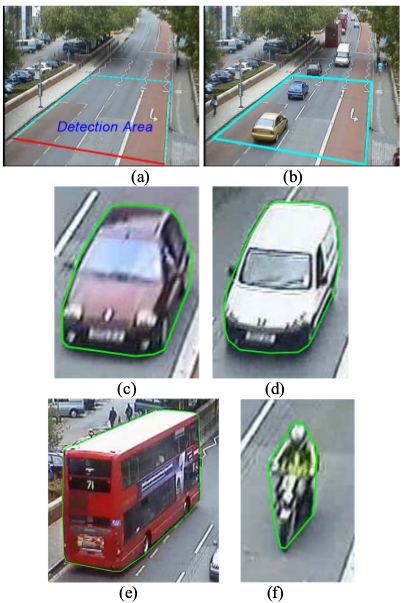
\includegraphics[width=0.4\textwidth]{figures/Estado_arte/svm_iphog.png}
		\caption{Detecciones del sistema de  Zezhi Chen and Tim Ellis~\cite{multi_shape_descriptor}}
		\label{fig.multi_shape_descriptor}
		\end{center}
\end{figure}

En las técnicas basadas en modelos 3D es necesario conocer los parámetros de la cámara que se emplee. En este caso tendremos una plantilla por cada clase y compararemos dicha plantilla con el objeto a clasificar para ver cual es la clase que más se le ajusta.
Wook-Sun Shin, Doo-Heon Song and Chang-Hun Lee~\cite{vehicle_classification_by_road} presenta  un  sistema  basado  en  plantillas  3D  que  no necesita una cámara calibrada. Este sistema se bada en los puntos de fuga de los carriles para reconstruir la forma 3D de cada vehículo. Un ejemplo de esta reconstrucción se puede ver en la Figura \ref{fig.3d_fuga}

\begin{figure}[H]
  \begin{center}
    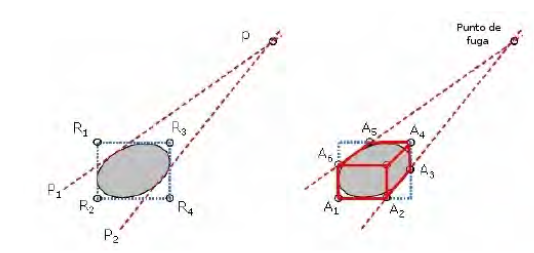
\includegraphics[width=0.6\textwidth]{figures/Estado_arte/3d_puntos_fuga.png}
		\caption{Reconstrucción 3D empleando puntos de fuga}
		\label{fig.3d_fuga}
		\end{center}
\end{figure}

Este sistema se basa en el algoritmo C4.5 de Quinlan~\cite{c4_5} a la hora de clasificar. Este algoritmo emplea la construcción de árboles de decisión para clasificar y aprender las siluetas de los vehículos. Un ejemplo de esta técnica puede verse en la Figura \ref{fig.c4_5}.

\begin{figure}[H]
  \begin{center}
    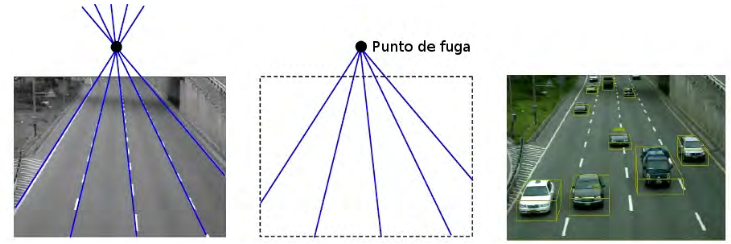
\includegraphics[width=1\textwidth]{figures/Estado_arte/c4_5.png}
		\caption{Clasificación de vehículos basada en modelos 3D construidos mediante el uso de puntos de fuga}
		\label{fig.c4_5}
		\end{center}
\end{figure}

Buch et al.~\cite{3dhog_article} presentaron un sistema que combinaba plantillas 3D con \acrshort{hog} para clasificar los diferentes vehículos y los peatones. Este sistema se llama 3DHOG, y en el aplican descriptores \acrshort{hog} a plantillas 3D que definen los vehículos. Para cada categoría se define una plantilla 3D que permita definirla. En la Figura ~\ref{fig.3dhog} se puede ver un ejemplo de dichas plantillas.

\begin{figure}[H]
  \begin{center}
    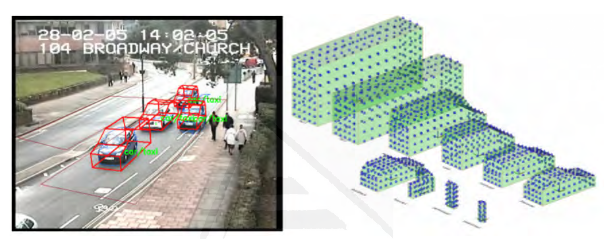
\includegraphics[width=0.8\textwidth]{figures/Estado_arte/3dhog.png}
		\caption{Plantillas 3DHOG para la clasificación de vehículos}
		\label{fig.3dhog}
		\end{center}
\end{figure}

En este sistema es necesario un previo entrenamiento. A la hora de realizar las clasificaciones se proyectan las plantillas 3D sobre los vehículos detectados y se les aplica transformaciones afines para ajustarlas al vehículo en cuestión. Tras esto se calculan sus histograma 3DHOG y se comparan con los que se han aprendido en la fase de entrenamiento. Esta reconstrucción de los histogramas 3DHOG puede verse en la Figura ~\ref{fig.3d_fuga}.

\begin{figure}[H]
  \begin{center}
    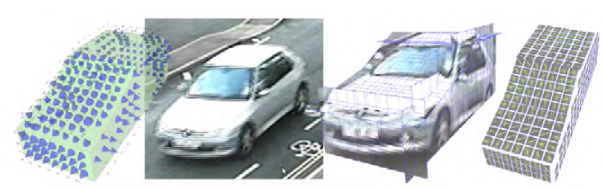
\includegraphics[width=0.7\textwidth]{figures/Estado_arte/3dhog_plantilla.png}
		\caption{Reconstrucción  del  histograma  3DHOG}
		\label{fig.3dhog_histograma}
		\end{center}
\end{figure}

Tal y como se ha comentado en la Seccion ~\ref{ap.deteccion_vehiculos} actualmente se ha extendido mucho el uso de Deep Learning tanto para la detección como para la clasificación de objetos. 
A.F. Granados y J.I. Marin.H~\cite{deteccion_flujo_vehicular} extraen los descriptores de Fourier de los vehículos detectados y los clasifican mediante una red neuronal. Dicha red neuronal consta de cuatro capas: una capa deentrada con una neurona por característica, dos capas ocultas con siete neuronas cada una y una capa de salida con una neurona clase. 


\section{Seguimiento de vehículos}

El seguimiento es la localización de un objeto a medida que va moviéndose por la imagen. Para el ser humano es una tarea muy sencilla, pero para la visión artificial se trata de un tema complejo, pues pueden cambiar muchas características en el objeto  a medida que avanza en la imagen. Tales como la forma, la iluminación, el tamaño, cambios en la perspectiva, oclusiones, movimiento de la cámara, etc.

Las técnicas más empleadas en el seguimiento de vehículos son:

\begin{itemize}
    \item Seguimiento basado en regiones
    \item Seguimiento basado en características
    \item Seguimiento basado en modelos
\end{itemize}

Las ténicas basadas en las regiones se centran en el seguimiento de regiones conexas del objeto. Normalmente la propiedad que suele emplearse es el color. En los diferentes artículos publicados se puede ver el uso de diferentes espacios de color como RGB, el espacio CEI lab o CEI LUV, el espacio HSV, etc. Lo más común es el uso de histogramas de color que nos permiten representar las regiones. Estas ténicas fueron introducidas por D. Comaniciu, V. Ramesh and P. Meer~\cite{kernel_based_object}. El seguimiento se basa en la comparación de los histogramas de las nuevas imágenes con el histograma de las regiones de interés calculadas en imágene sprevias. Para ver el parecido entre los histogramas se emplea una medida similar a la distancia de Bhattacharyya y mean-shift para optimizar la selección del candidato.

Stefan Duffner and Christophe Garcia~\cite{pixeltrack} presentó un algoritmo llamado PixelTrack, el cual combina la transformada de Hough con un modelo genérico de detección de fondo. Para ello necesita inicializar una ventana sobre el objeto. Gracias a esta técnica son capaces de seguir objetos en tiempo real con fondo cambiante, oclusiones y condiciones desfavorables.
Lili Huang and M. Barth~\cite{real_time_vehicle} plantean un algoritmo para llevar a cabo el seguimiento de vehículos y la resolución de oclusiones. En este algoritmo emplean un modelo de color basado en mean-shift para identificar a que vehículo pertenece cada parche de 3x3 píxeles cuando existe una oclusión.

El seguimiento basado en características, tal y como su nombre indica se centra en seguir los objetos en función a las características que se crean oportunas. Cada autor hace uso de unas características. Entre estas características tenemos puntos característicos como esquinas, el perímetro del objeto, sus dimensiones, etc. Si lo comparamos con el seguimiento basado en regiones podemos ver que es más robusto, pues en el caso de las regiones trataban de seguir el objeto en función del color o la textura, lo cual es muy suceptible ante el cambio de iluminación. Entre las técnicas más empleadas en este ámbito podemos encontrar \acrfull{sift}(D.G. Lowe~\cite{article_sift}), \acrfull{klt} (J. Shi and C. Tomasi~\cite{article_klt}). Otra ténica muy empelada en la literatura es \acrshort{hog}(Dalal and Bill Triggs~\cite{hog_paper}), la cual en muchas ocasiones ha sido combinada con \acrshort{svm}, tal y como se ha comentado en la seccion anterior, Zezhi Chen and Tim Ellis~\cite{multi_shape_descriptor} ya hicieron uso de ambos métodos.


El seguimiento basado en modelos trata de beneficiarse del conocimiento que tenemos de los objetos para poder realizar plantillas 2D y 3D para detectar objetos en la imagen y poder realizar su seguimiento. M.J. Leotta and J.L. Mundy~\cite{vehicle_surveillance_3d} emplean esta técnica para detectar vehículos haciendo uso de una plantilla deformable que se ajusta para identificar diferentes formas de vehículos. En la literatura también se ha combinado esta técnica con filtros de Kalman.


\section{Bases de Datos para la detección de vehículos}
\label{sec:dataset}

La detección de vehículos pretende encontrar un vehículo en una imagen o en un vídeo y determinar qué tipo de vehículo es. Dado que queremos encontrar el vehículo en cuestión bajo diferentes circunstancias, es decir, en diferentes entornos y diferentes iluminaciones, necesitaremos entrenar el modelo con un conjunto de imágenes representativo. Por este motivo, a lo largo de los últimos años han surgido diferentes datasets con el fin de solucionar este problema.

\subsection{GRAM Road-Traffic Monitoring}

GRAM Road-Traffic Monitoring (GRAM-RTM) \cite{gram-tracking} \cite{gram} es un conjunto de datos para el seguimiento de vehículos en tiempo real. Consiste en 3 secuencias de video (Figura \ref{fig.gram}), grabadas bajo diferentes condiciones y con diferentes plataformas.

El primer video, llamado M-30 (7520 \textit{frames}), se grabó en un día soleado con una cámara Nikon Coolpix L20, con una resolución de 800 x 480 @ 30 fps. La segunda secuencia, llamada M-30-HD (9390 \textit{frames}), se grabó en una ubicación similar pero durante un día nublado, y con una cámara de alta resolución: una Nikon DX3100 a 1200 x 720 @ 30 fps. La tercera secuencia de video, llamada Urban1 (23435 \textit{frames}), se grabó en una intersección concurrida con una cámara de tráfico de video vigilancia con una resolución de 600 x 360 @ 25fps.

Todos los vehículos en el conjunto de datos GRAM-RTM fueron anotados manualmente. Este conjunto posee las siguientes categorías de clases: coches, camiones, furgonetas y camiones grandes. El número total de objetos diferentes en cada secuencia es: 256 para M-30, 235 para M-30-HD y 237 para Urban1. Todas las anotaciones en el conjunto GRAM-RTM se crearon en un formato XML compatible con PASCAL VOC.

\begin{figure}
\begin{center}
	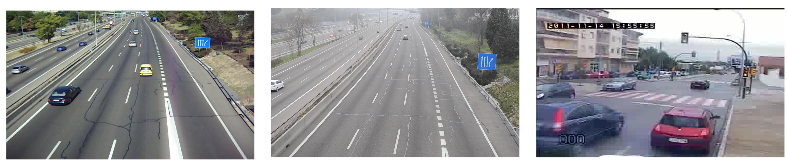
\includegraphics[width=1\textwidth]{figures/Estado_arte/gram.png}
   \caption{Imágenes de ejemplo del dataset GRAM Road-Traffic Monitoring}
	\label{fig.gram}
\end{center}
\end{figure}

\subsection{BIT-Vehicle Dataset}

El conjunto de datos BIT-Vehicle \cite{bit} contiene 9850 imágenes de vehículos. Contiene imágenes con tamaños de 1600 x 1200 y 1920 x 1080. Estas imágenes (Figura \ref{fig.bit}) fueron capturadas desde dos cámaras en diferentes momentos y lugares. Las imágenes contienen cambios en las condiciones de iluminación, la escala, el color de la superficie de los vehículos y el punto de vista. Las partes superior o inferior de algunos vehículos no están incluidas en las imágenes debido a la demora en la captura y al tamaño del vehículo. 

En cada imagen puede haber uno o dos vehículos y la ubicación de cada vehículo está previamente anotada. Además, el conjunto de datos se puede utilizar para evaluar el rendimiento de la detección de vehículos.

Los vehículos del conjunto de datos se dividen en seis categorías: bus, microbus, minifurgoneta, Sedan, SUV y camión. El número de vehículos por tipo de vehículo es de 558 para bus, 883 para microbus, 476 para minifurgoneta, 5922 para Sedan, 1392 para SUV, y 82 para camiones.

\begin{figure}[H] 
\begin{center}
	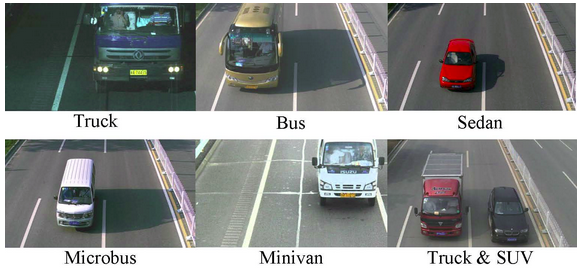
\includegraphics[width=0.9\textwidth]{figures/Estado_arte/bit.png}
   \caption{Imágenes de ejemplo del dataset BIT-Vehicle}
	\label{fig.bit}
\end{center}
\end{figure}

\subsection{CarND-Vehicle-Detection}

CarND-Vehicle-Detection \cite{carnd1} es un proyecto dedicado a la detección de vehículos en vídeo, por ello crearon dos conjuntos de datos que se pueden encontrar en \cite{carnd2}.

El \textit{dataset} 1 incluye datos de conducción en Mountain View California y las ciudades vecinas durante el día. Contiene más de 65000 etiquetas en 9423 imágenes almacenadas por una cámara de investigación Point Grey que se ejecuta a una resolución máxima de 1920x1200 a 2Hz. El conjunto de datos fue anotado mediante CrowdAI utilizando una combinación entre aprendizaje automático y el trabajo de personas. Este conjunto de datos ocupa un total de 1.5 GB, y las clases que contiene son: coche, camión y peatón.

El \textit{dataset} 2 es similar al conjunto de datos 1, pero contiene campos adicionales para la oclusión y una etiqueta adicional para los semáforos. El conjunto de datos fue anotado en su totalidad por humanos usando Autti y es un poco más grande que el anterior con 15000 imágenes (ocupa 3.3 GB). Este conjunto incluye las clases: coche, camión, peatón y farolas.
\begin{figure}[H] 
\begin{center}
	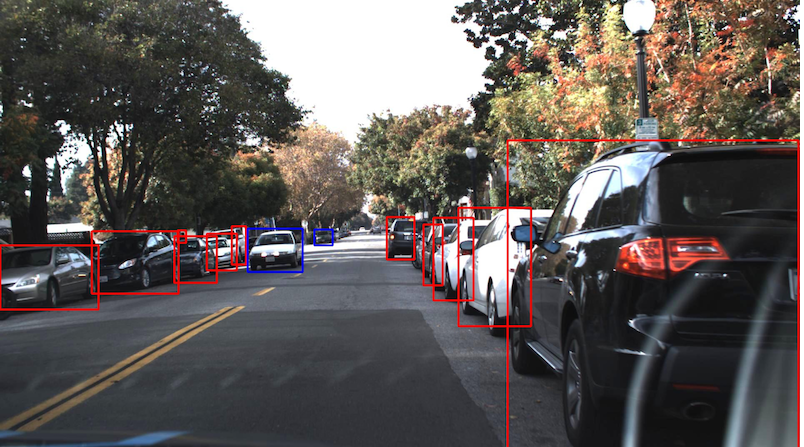
\includegraphics[width=0.8\textwidth]{figures/Estado_arte/carnd_dataset2.png}
   \caption{Imágenes de ejemplo del dataset 2 de CarND-Vehicle-Detection}
	\label{fig.carnd}
\end{center}
\end{figure}
